\section{Résultats et perspectives}
\paragraph{}
Dans cette section nous allons présenter les différents résultats obtenus dans le cadre de nos travaux. Dans les légendes des graphes présentés, \texttt{rk\_i} et \texttt{bdf\_i} désignent les méthodes RK et BDF d'ordre i, et \texttt{taylor\_exp\_i} et \texttt{rosen\_exp\_i} les méthodes exponentielles classiques et de Rosenbrock d'ordre i. Pour ne pas introduire de source d'erreur, les méthodes exponentielles sont réalisées sans utiliser de méthode d'approximation de type Krylov, comme présenté précédemment.Le code python utilisé est disponible sur le dépot GitHub \cite{repo_git}.
\begin{figure}
    \centering
    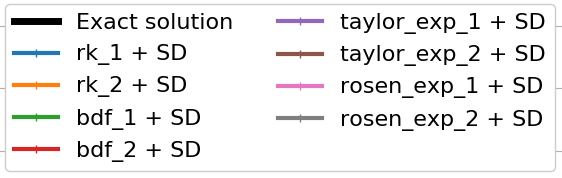
\includegraphics[width=0.5\textwidth]{images/results/legend.png}
    \caption{Légende des graphes}
    \label{fig:legend}
\end{figure}
\paragraph{}
Les graphes présentés dans cette partie utilisent la légende présentée en figure \ref{fig:legend}.


\subsection{Équation différentielles ordinaire}
    \paragraph{}
    Tout d'abord, nous avons regardé les différentes méthodes temporelles sur des EDO, afin de les étudier plus facilement et de manière plus exhaustive (c'est à dire sur plus de problèmes).
        
    \subsubsection{Cas linéaire}
    \paragraph{}
    Premièrement, nous allons nous intéresser à l'équation harmonique :
    \begin{equation}
        \left\{
        \begin{aligned}
            &\ddot{y} + y = 0 \\
            &\left(y, \dot{y}\right)_{t = 0} = \left(1, 0\right)
        \end{aligned}
        \right.
        \Longleftrightarrow
        \left\{
        \begin{aligned}
            &\dot{Y} = \begin{bmatrix}0 & 1\\-1 & 0\end{bmatrix}Y \\
            &Y_{t = 0} = \begin{pmatrix}1\\0\end{pmatrix}\\
            &Y = \begin{pmatrix}y\\\dot{y}\end{pmatrix}
        \end{aligned}
        \right.
    \label{eq:edo_harmonique}
    \end{equation}
    La solution de cette équation est la fonction cosinus.
    \begin{figure}
        \centering
        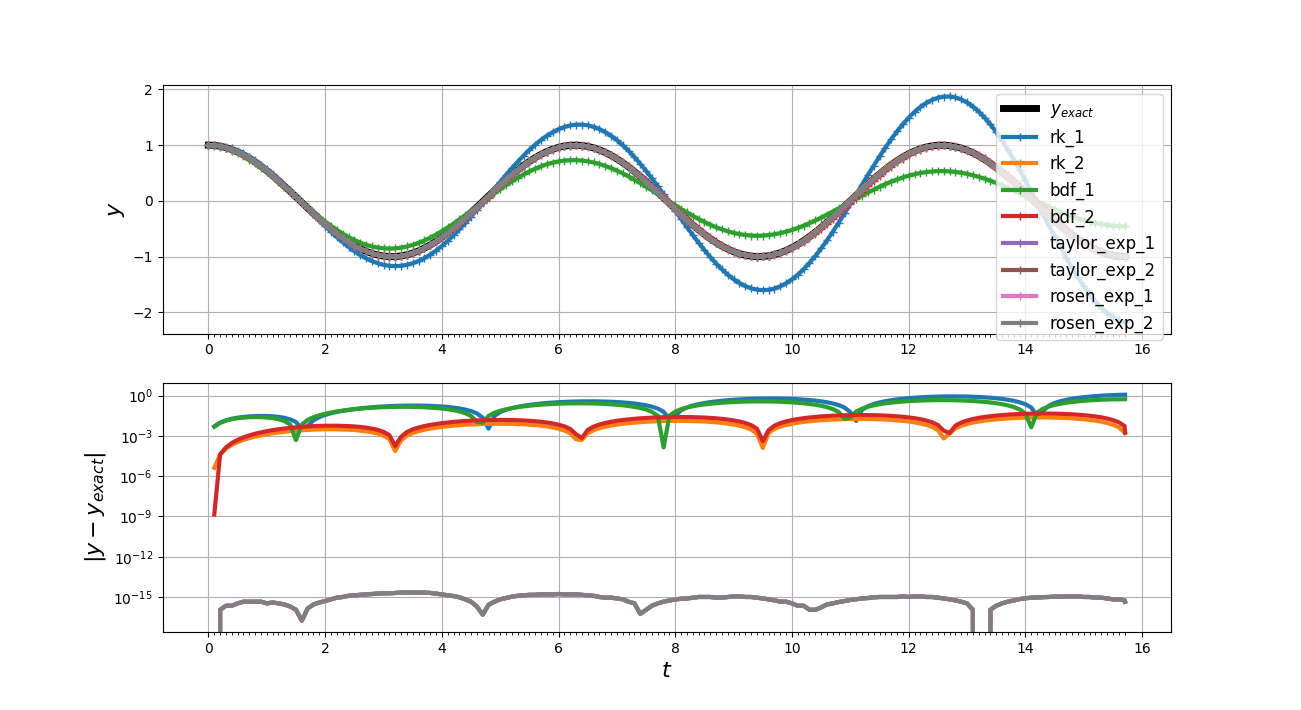
\includegraphics[width=\textwidth]{images/results/edo_sine.png}
        \caption{Résultats pour l'équation \ref{eq:edo_harmonique}, avec $\Delta t = 0.1$}
        \label{fig:edo_harmonique}
    \end{figure}
    \paragraph{}
    Sur la figure \ref{fig:edo_harmonique}, on voit les différents résultats calculés par les deux premiers ordres de chacune des méthodes (RK, BDF, exponentielles de Taylor et de Rosenbrock). La figure du haut représente la solution calculée en fonction du temps, et celle du bas l'écart à la solution théorique, en échelle semi-log. Nous pouvons y faire plusieurs observations :
    \begin{itemize}
        \item les courbes des différentes méthodes exponentielles sont toutes confondues
        \item les premiers ordres des méthodes RK et BDF s'éloignent de la solution exacte, en divergeant pour la méthode RK1 et en tendant vers 0 pour la méthode BDF1
        \item toutes les autres solutions calculées semblent confondues avec la solution théorique, y compris les premiers ordres des méthodes exponentielles
        \item en regardant le graphe du bas, on voit que l'erreur des méthodes RK2 et BDF2 sont du même ordre de grandeur, plus bas que celle des ordres 1 correspondants mais bien supérieurs à l'erreur des méthodes exponentielles, tout ordre confondu
    \end{itemize}
    \begin{figure}
        \centering
        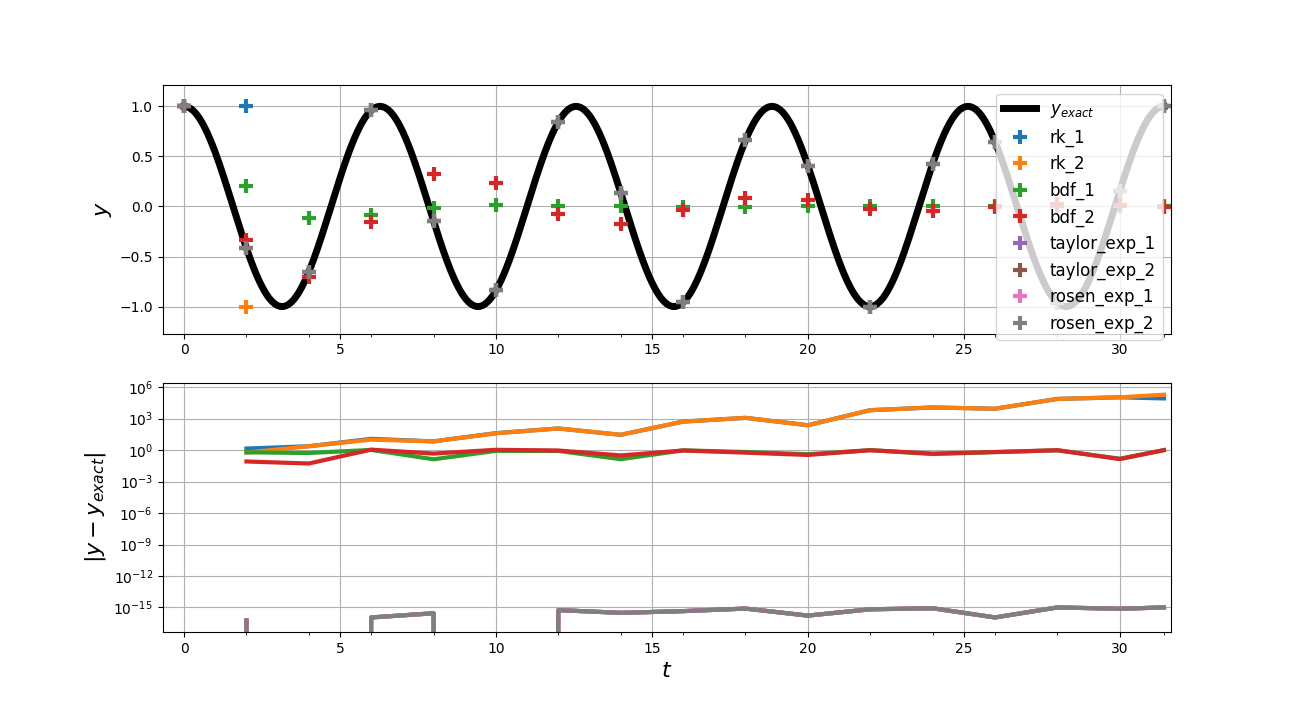
\includegraphics[width=\textwidth]{images/results/edo_sine_large_dt.png}
        \caption{Résultats pour l'équation \ref{eq:edo_harmonique}, avec $\Delta t = 2$}
        \label{fig:edo_harmonique_2}
    \end{figure}
    \paragraph{}
    En regardant bien les équations, on se rend compte que, puisque cette équation à un second membre linéaire, une méthode exponentielle est censée calculer la solution exacte, inconditionnellement. Ainsi, nous avons résolu la même équation, mais avec un pas de temps bien supérieur. Le résultat de cette simulation est représenté sur la figure \ref{fig:edo_harmonique_2}. Cette fois, on ne voit plus les méthodes RK, qui divergent rapidement vers l'infini. On peut vérifier le constat précédent : alors que les méthodes BDF s'écrasent vers 0, les méthodes exponentielles, qui sont à nouveau confondues sur le graphe, calculent la solution presque exactement. La faible erreur que l'on observe est introduite par les calculs matriciels intervenant dans les méthodes exponentielles, et non par des erreurs de la méthode.


    \subsubsection{Cas raide}
    \paragraph{}
    Le deuxième cas que nous présentons ici est un cas non linéaire, dit \emph{raide}, présenté dans l'article \cite{stiff_equation}.
    L'équation résolue est :
    \begin{equation}
        \begin{split}
            \left\{
            \begin{aligned}
                &\dot{y} = -50\left(y - \cos\left(t\right)\right) \\
                &y\left(0\right) = 0
            \end{aligned}
            \right.
        \end{split}
    \label{eq:raide}
    \end{equation}
    Cette équation admet pour solution $y\left(t\right) = \frac{50}{2501}\sin\left(t\right)+\frac{2500}{2501}\cos\left(t\right) -\frac{2500}{2501}e^{-50t}$.
    \begin{figure}
        \centering
        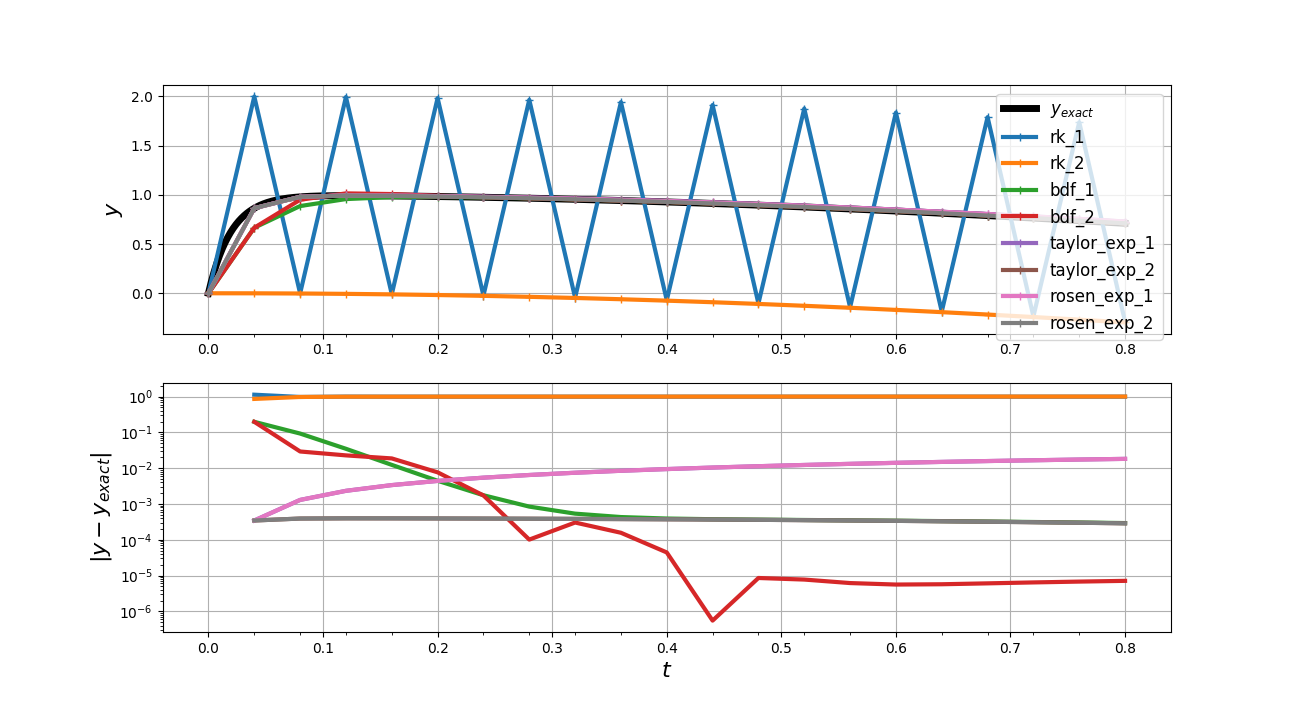
\includegraphics[width=\textwidth]{images/results/edo_raide.png}
        \caption{Résultats pour l'équation \ref{eq:raide}, avec $\Delta t = 0.04$}
        \label{fig:edo_raide}
    \end{figure}
    \paragraph{}
    Sur la figure \ref{fig:edo_raide}, on voit à nouveau la solution calculée par les différentes méthodes, ainsi que l'écart à la solution analytique. On y fait les observations suivantes :
    \begin{itemize}
        \item les courbes des méthodes exponentielles de même ordre sont à nouveau confondues
        \item les méthodes explicites (RK) ne parviennent pas à évaluer une solution correcte avec un tel pas de temps, alors que les méthodes implicites (BDF) et exponentielles y arrivent
        \item pour les méthodes exponentielles et BDF, on voit que les ordres supérieurs sont plus précis
    \end{itemize}
    \paragraph{}
    Grâce à ce cas, on peut donc voir que les méthodes exponentielles permettent aussi de résoudre des problèmes non linéaires, et même raides.

    
    \subsubsection{Cas non linéaire}
    \paragraph{}
    L'équation résolue ici est :
    \begin{equation}
        \begin{split}
            \left\{
            \begin{aligned}
                &\dot{y} = y^2 \\
                &y\left(0\right) = 0.1
            \end{aligned}
            \right.
        \end{split}
    \label{eq:nonlinear}
    \end{equation}
    Cette équation admet pour solution $y\left(t\right) = \frac{0.1}{1 - 0.1t}$. Sa particularité réside dans le fait qu'elle est fortement non linéaire, et diverge en un temps fini (ici $t = 10$). Pour l'étudier, on utilise une discrétisation temporelle irrégulière : on va réduire le pas de temps à mesure qu'on s'approche de la divergence pour mieux calculer la solution. La discrétisation utilisée ici est $t_{0\leq i\leq 19} = 10\left(1 - 10^{-i/19}\right)$.
    \begin{figure}
        \centering
        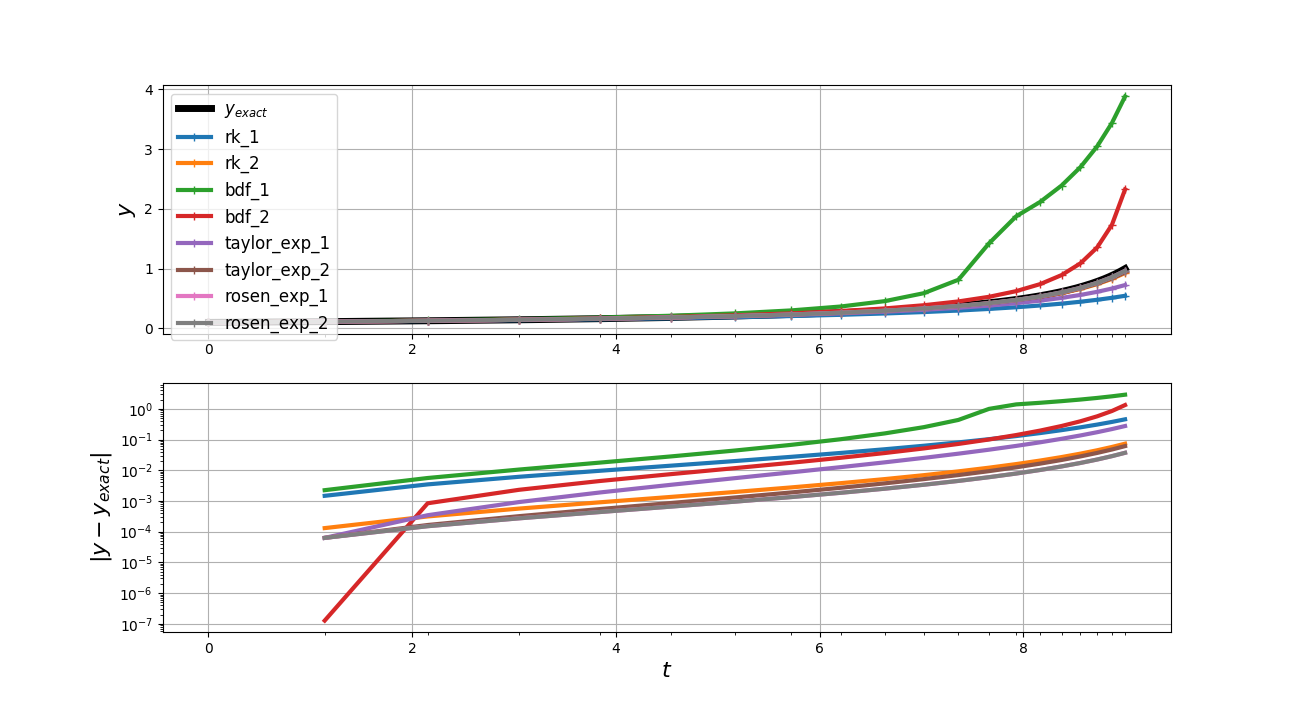
\includegraphics[width=\textwidth]{images/results/edo_nonlinear.png}
        \caption{Résultats pour l'équation \ref{eq:nonlinear}, calculée aux instants $t_{0\leq i\leq 19} = 10\left(1 - 10^{-i/19}\right)$}
        \label{fig:edo_non_lineaire}
    \end{figure}
    \paragraph{}
    Sur la figure \ref{eq:nonlinear}, on affiche les résultats obtenus avec les mêmes méthodes que précédemment. On y observe les résultats suivants :
    \begin{itemize}
        \item cette fois-ci ce sont les méthodes BDF qui s'écartent beaucoup de la solution
        \item on a toujours que la précision augmente avec l'ordre de la méthode
        \item les méthodes de Rosenbrock sont meilleures que les méthodes de Taylor classiques, puisqu'elles actualisent la partie linéaire qu'elles prennent en compte à chaque pas de calcul
        \item puisque la partie linéaire prise en compte par les méthodes de Taylor classique reste la même le long du calcul et s'éloigne de la réelle partie linéaire de la solution, ces méthodes tendent vers les méthodes RK du même ordre (sur le graphe des erreurs, la courbe violette tend vers la bleue, et la marron tend vers la orange)
        \item les deux méthodes de Rosenbrock restent équivalentes, puisque la non linéarité est elle linéaire (la hessienne du membre de droite est constante)
    \end{itemize}
    \paragraph{}
    Cette fois encore, les méthodes exponentielles restent meilleures que les autres méthodes du même ordre.
    
    \paragraph{}
    Finalement, ces cas tests sur des EDO ont permis de montrer que les méthodes exponentielles sont performantes à la fois sur les domaines d'utilisation des méthodes explicite, et aussi sur ceux des méthodes implicites. Et dans le meilleur des cas, le cas linéaire, elles permettent de résoudre exactement le problème donné.
    
	
\subsection{Équation aux dérivées partielles}
    \paragraph{}
    L'étude préliminaire avec des EDO permet de mieux comprendre les méthodes exponentielles, mais l'intérêt du client se porte sur les EDP. Pour tester les méthodes temporelles sur des EDP, nous utilisons un schéma spatial de Différences Spectrales (SD) d'ordre 2 en 1D, sur un intervalle avec des conditions aux limites périodiques.

    \subsubsection{Problème d'advection - diffusion}
    \paragraph{}
    Tout d'abord, le problème étudié est celui de l'advection - diffusion :
    \begin{equation}
        \frac{\partial y}{\partial t} + c\frac{\partial y}{\partial x} = d\frac{\partial^2 y}{\partial^2 x}
        \Longleftrightarrow \frac{\partial y}{\partial t} + \frac{\partial}{\partial x}\left(cy - d\frac{\partial y}{\partial x}\right) = 0
    \label{eq:edp_advection_diffusion}
    \end{equation}
    avec les paramètres $c$ et $d$ constants, et $d \ge 0$.
    
    \begin{figure}
        \centering
        \begin{subfigure}{.5\textwidth}
            \centering
            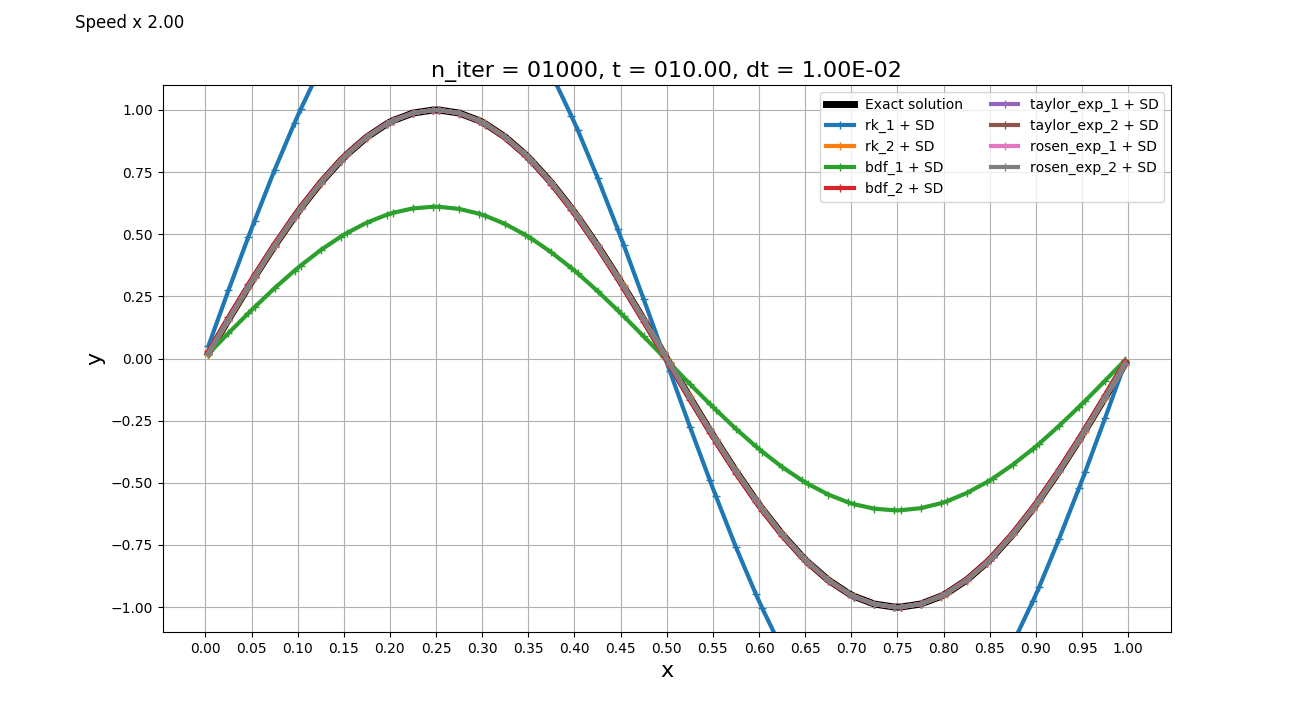
\includegraphics[width=\textwidth]{images/results/edp_advection_1.png}
            \caption{t = 10}
        \label{fig:edp_advection_1}
        \end{subfigure}
        \begin{subfigure}{.5\textwidth}
            \centering
            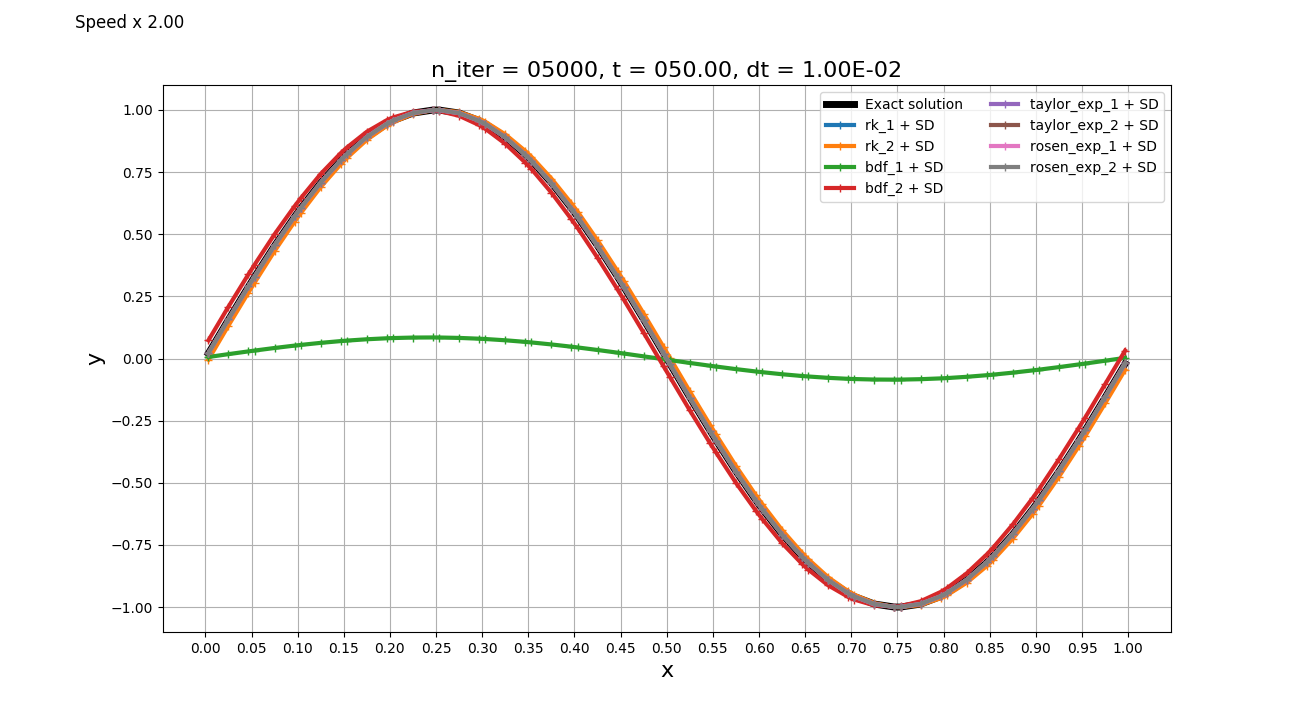
\includegraphics[width=\textwidth]{images/results/edp_advection_2.png}
            \caption{t = 50}
        \label{fig:edp_advection_2}
        \end{subfigure}%
        \begin{subfigure}{.5\textwidth}
            \centering
            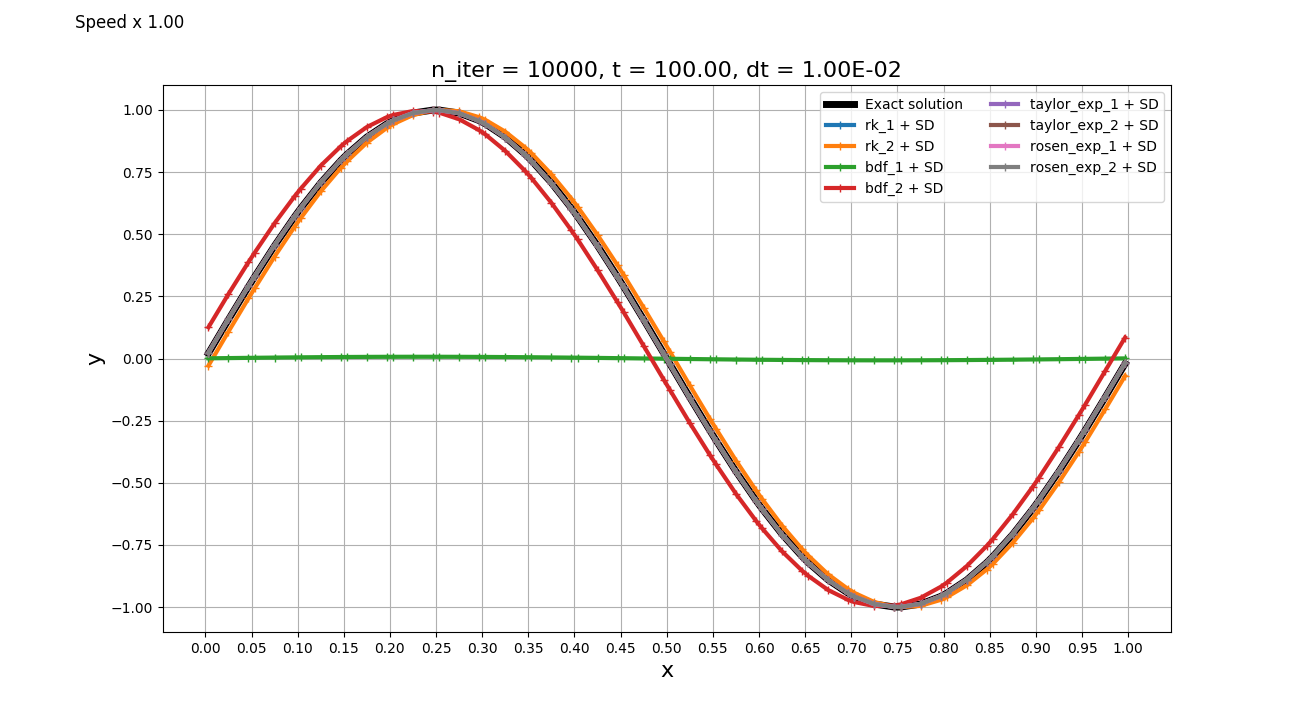
\includegraphics[width=\textwidth]{images/results/edp_advection_3.png}
            \caption{t = 100}
        \label{fig:edp_advection_3}
        \end{subfigure}
    \caption{Solutions calculées pour le problème d'advection pure ($c = 0.5$, $d = 0$), avec un schéma spatial SD d'ordre 2 et un pas de temps $\Delta t = 0.01$ (CFL = 0.746)}
    \label{fig:edp_advection}
    \end{figure}
    \paragraph{}
    Tout d'abord, avec une équation d'advection pure ($c = 0.5$, $d = 0$), on regarde les résultats présentés sur la figure \ref{fig:edp_advection}.
    \begin{itemize}
        \item Sur la figure \ref{fig:edp_advection_1}, on voit qu'après 1000 itérations la méthode RK1 commence à diverger, et la méthode BDF1 à s'écraser vers 0.
        \item Sur la figure \ref{fig:edp_advection_2}, après 5000 itérations, la méthode BDF1 est très proche de 0, et on voit que les méthodes RK2 et BDF2 commencent à se séparer de la solution théorique.
        \item Sur la figure \ref{fig:edp_advection_3}, après 10000 itérations, les méthodes RK2 et BDF2 ont un déphasage bien visible par rapport à la solution théorique.
        \item Tout le long du calcul, les méthodes exponentielles sont indistinguables de la solution théorique.
    \end{itemize}
    \begin{figure}
        \centering
        \begin{subfigure}{.5\textwidth}
            \centering
            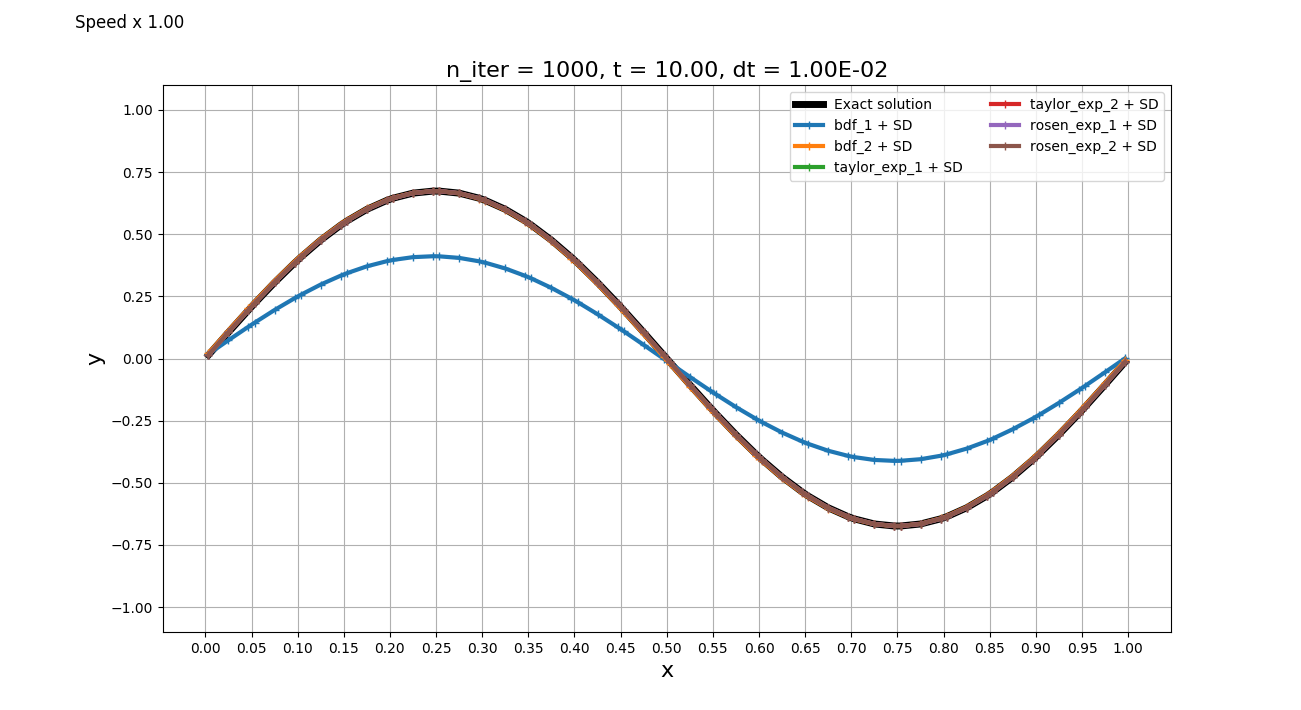
\includegraphics[width=\textwidth]{images/results/edp_adv_diff_cfl_1.png}
            \caption{$\Delta t = 0.01$ (CFL = 0.746)}
        \label{fig:edp_adv_diff_cfl_1}
        \end{subfigure}%
        \begin{subfigure}{.5\textwidth}
            \centering
            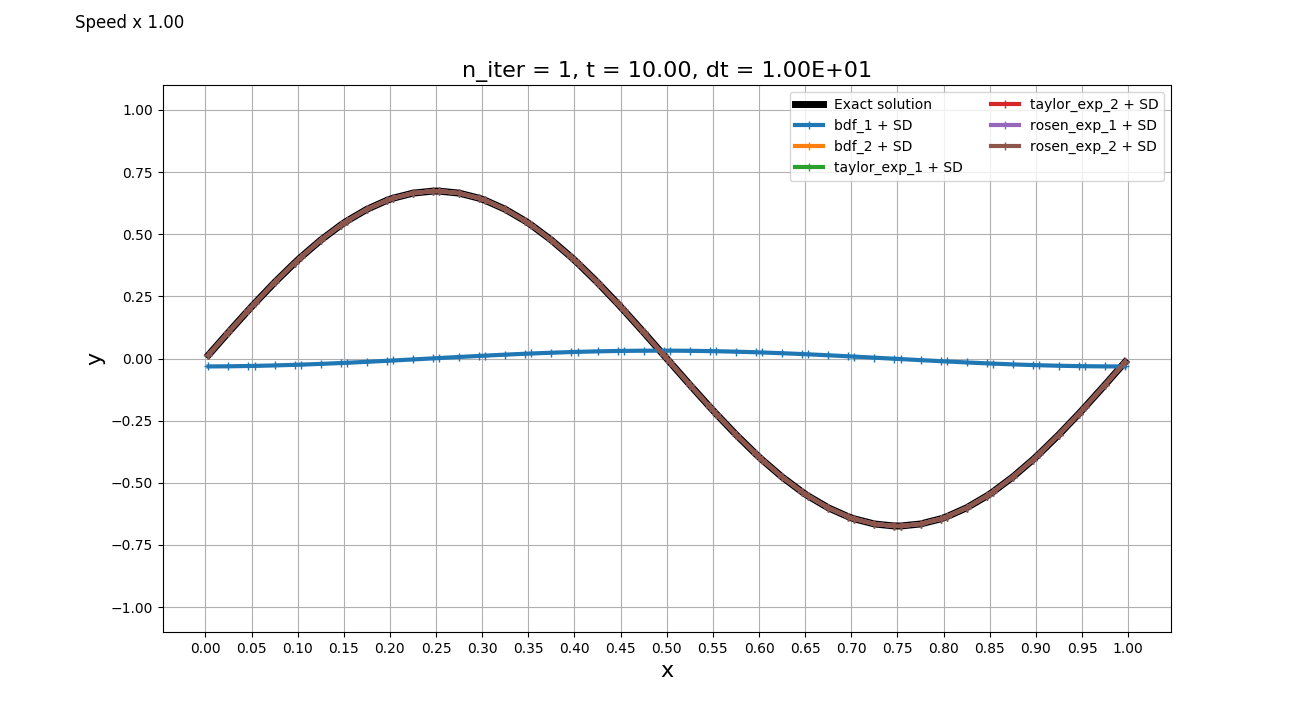
\includegraphics[width=\textwidth]{images/results/edp_adv_diff_cfl_2.png}
            \caption{$\Delta t = 10$ (CFL = 746.41)}
        \label{fig:edp_adv_diff_cfl_2}
        \end{subfigure}
        \caption{Solutions calculées pour le problème d'advection diffusion ($c = 0.5$, $d = 0.001$), avec un schéma spatial SD d'ordre 2, à t = 10 et pour différentes valeurs du pas de temps}
    \label{fig:edp_adv_diff_cfl}
    \end{figure}
    \paragraph{}
    Tout comme dans le cas de l'EDO linéaire vue précédemment, les méthodes exponentielles sont sensées résoudre ce problème d'advection de manière exacte, puisque la méthode SD donne un membre de droite linéaire pour des problèmes d'advection diffusion. Nous avons pu vérifier ceci grâce au cas présenté en figure \ref{fig:edp_adv_diff_cfl}. On y voit que :
    \begin{itemize}
        \item pour une faible valeur du nombre CFL la méthode BDF d'ordre 2 peut calculer une bonne approximation de la solution, sur la figure \ref{fig:edp_adv_diff_cfl_1}
        \item pour une plus grande valeur du nombre CFL la méthode BDF2 ne peut plus calculer d'approximation de la solution, sur la figure \ref{fig:edp_adv_diff_cfl_2}
        \item pour n'importe quel nombre de CFL arbitrairement grand, les méthodes exponentielles sont indistinguables de la solution théorique
    \end{itemize}
    
    \subsubsection{Équation de Burgers}
    \paragraph{}
    Les méthodes exponentielles résolvent ainsi très facilement les équations différentielles où le membre de droite est linéaire. Pour pouvoir conclure quand à leur performances, il faut d'abord les tester sur un problème non linéaire. Pour cela nous avons développé un code SD pour modéliser l'équation de Burgers :
    \begin{equation}
        \frac{\partial y}{\partial t} + y\frac{\partial y}{\partial x} = d\frac{\partial^2 y}{\partial^2 x}
        \Longleftrightarrow \frac{\partial y}{\partial t} + \frac{\partial}{\partial x}\left(\frac{y^2}{2} - d\frac{\partial y}{\partial x}\right) = 0
    \label{eq:burgers}
    \end{equation}
    
    \begin{figure}
        \centering
        \begin{subfigure}{.5\textwidth}
            \centering
            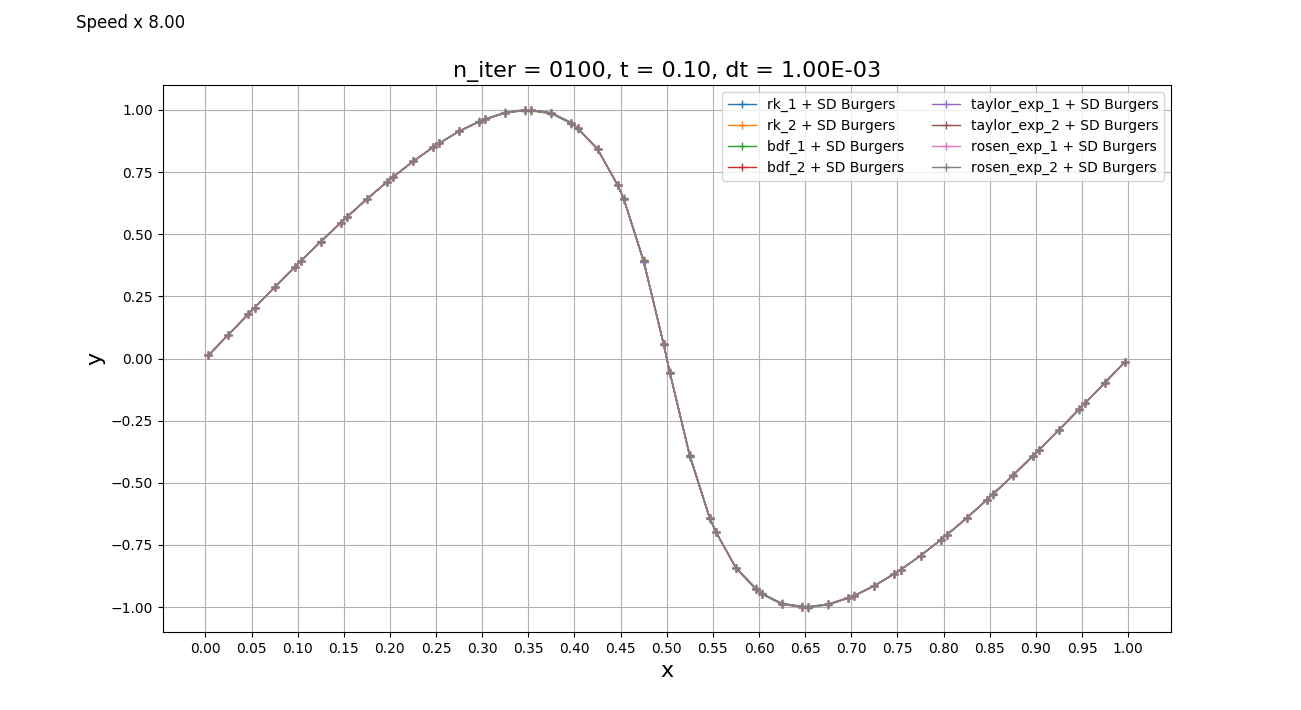
\includegraphics[width=\textwidth]{images/results/edp_burgers_1.png}
            \caption{t = 0.1}
        \label{fig:edp_burgers_1}
        \end{subfigure}%
        \begin{subfigure}{.5\textwidth}
            \centering
            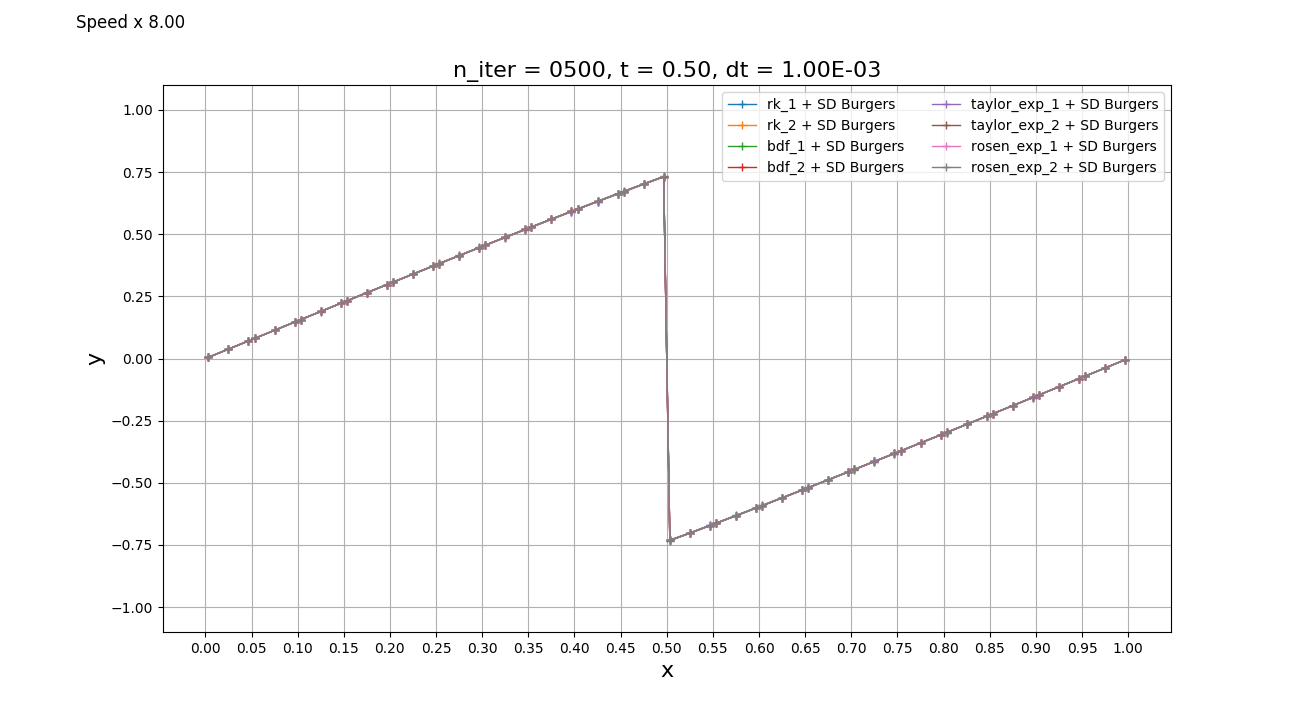
\includegraphics[width=\textwidth]{images/results/edp_burgers_2.png}
            \caption{t = 0.5}
        \label{fig:edp_burgers_2}
        \end{subfigure}
        \caption{Solutions calculées pour le l'équation de Burgers (equation \ref{eq:burgers}) non visqueuse ($d = 0$), avec un schéma spatial SD d'ordre 2, pour $\Delta t = 0.001$ (CFL = 0.149)}
    \label{fig:edp_burgers}
    \end{figure}
    \paragraph{}
    Sur la figure \ref{fig:edp_burgers}, on peut voir que les méthodes exponentielles donnent également des résultats satisfaisants sur des problèmes où le membre de droite n'est pas linéaire. En effet sur cette figure, toutes les courbes sont confondues. Il n'existe pas de solution analytique à l'équation \ref{eq:burgers} avec un sinus comme condition initiale sur un segment avec des conditions aux limites périodiques. Nous avons donc vérifié, avec des schémas connus, des pas de temps faibles et des maillages fins, que la solution affichée sur la figues \ref{fig:edp_burgers} est bien celle vers laquelle on tend (et c'est donc à priori la solution exacte). En étant confondues dans ces autres solutions convergées, les méthodes exponentielles nous montrent qu'elles peuvent résoudre cette équation de Burgers.
    

\subsection{Conclusion et perspectives}

\paragraph{}
Cette étude nous aura permis de mieux appréhender les méthodes exponentielles, en mettant en valeurs leurs atouts par rapport aux méthodes plus classiques de type RK et BDF. Grâce aux EDO, nous avons pu étudier toutes ces méthodes sur des cas très variée. Cette première démarche aura montré que les méthodes exponentielles possèdent les qualités de ces deux autres types de méthodes, et peuvent même dans certains cas simple résoudre exactement un problème. La conclusion pourrait être formulée de la manière suivante : \emph{dans le pire des cas c'est une méthode classique (RK ou BDF) et dans le meilleur des cas c'est une méthode exacte}.

\paragraph{}
La seconde partie de l'étude concerne les EDP. Nous avons montré que les méthodes exponentielles sont tout à fait applicables dans la résolution de ce type de problèmes. Toujours sur les problèmes qui ont un second membre linéaire, les méthodes exponentielles sont imbattables car elles permettent d'utiliser n'importe quel pas de temps, c'est à dire de déterminer n'importe quel état aussi loin dans le temps que voulu, en une seule itération.

\paragraph{} 
Le plus grand défaut de ces méthodes temporelle reste leur coup de calcul : il est nécessaire de calculer des exponentielles de matrices, opération qui est très coûteuse d'un point de vue informatique. Pour contourner ce problème, nous nous sommes intéressé aux méthodes de Krylov, qui permettent d'accélérer énormément le calcul en offrant un compromis temps d'exécution - précision qui semble raisonnable.
